
%-------------------------------------------------------------------------------
%\section{Protocol}
%-------------------------------------------------------------------------------
\begin{figure*}[!th]
\begin{center}
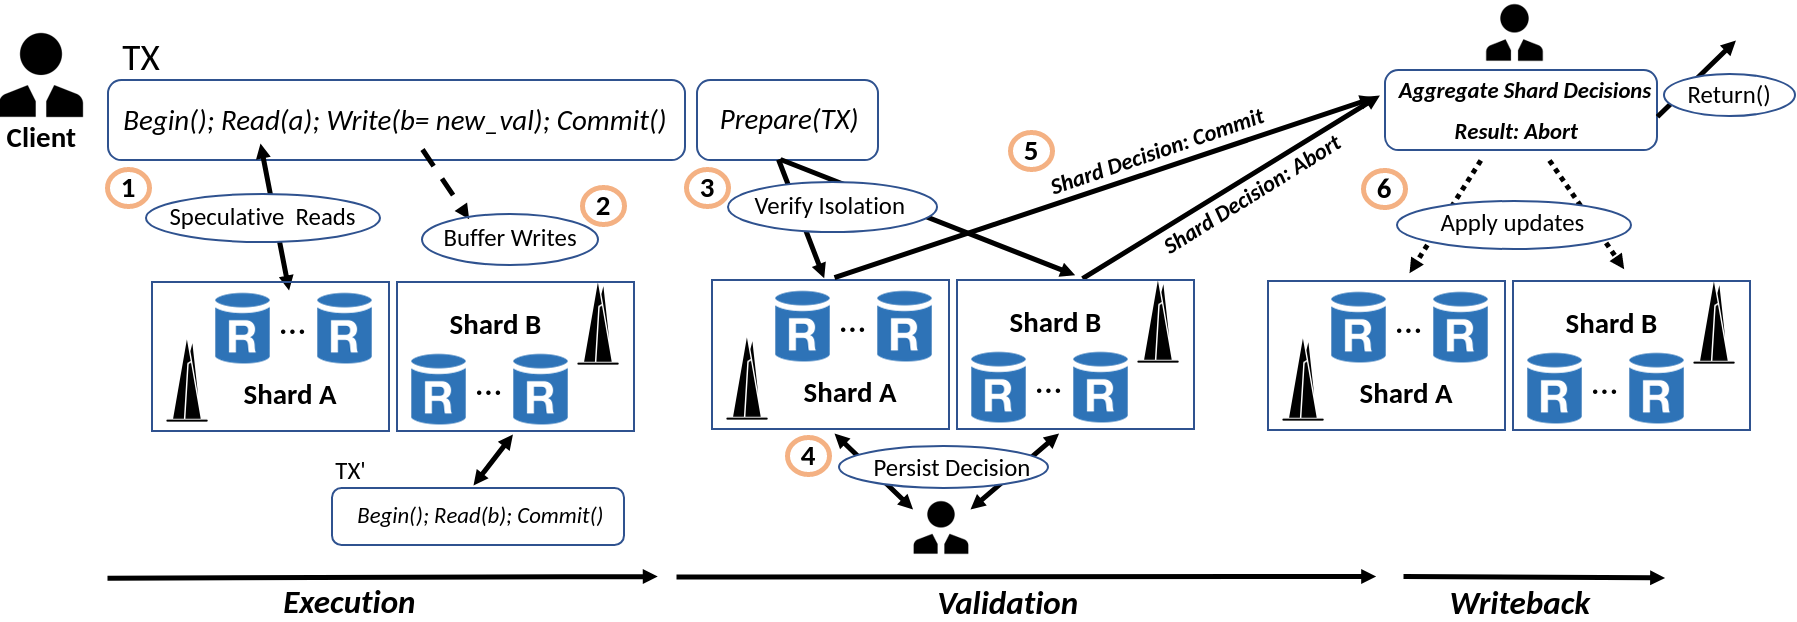
\includegraphics[width= \textwidth]{./figures/Archi.png}
\end{center}
\caption{{\em Transaction Lifecycle}. Clients execute remote reads (1) and buffer writes (2). For Committment, all involved shards verify isolation (3). If there are conflicting transactions (TX'), replicas in a shard (B) vote to Abort. A client persists a decision (4) that serves as Two-Phase-Commit Vote for each shard (5), and Commits a transaction if all shards vote to commit (6).}
\label{fig:Figure1}
\end{figure*}
\fs{cut figure if it is not useful} \nc{I don't figure hurts, but I don't think it helps much either}\la{I would tentatively remove it: we are probably going to need the space}

\sys is is a sharded and replicated transactional key-value store designed to be scalable and leaderless, and our architecture reflects this ethos. 

\par \textbf{Transaction Execution} Transaction execution is driven by clients (removing costly all-to-all communications amongst replicas) and consists of three phases. First, in an \textit{execution phase}, clients execute individual transactional operations. As is standard in optimistic databases, reads are submitted to remote replicas while writes are buffered locally. \sys{} supports \textit{interactive} and cross-shard transactions: clients can issue new operations based on the results of past operations to any shard in the system. \sys{} must additionally ensure that these read operations do not violate Byzantine independence. In a second \textit{validation phase}, invidual shards in \sys{} must validate whether committing the transaction would violate serializability. For performance, \sys{} allows invidiual replicas within a shard to process requests out of order. \sys{} must additionally ensure that Byzantine actors cannot cause spurious aborts. Finally, \sys{} aggregates each shard decision in a \textit{commit phase} \fs{decision phase? must rename writeback section} to determine the outcome of the transaction, notifies both application and replicas in the system of the decision, and, if the decision was to commit, makes the buffered writes persistent in the data store.  Importantly, the decision of whether each transaction commits or aborts must be preserved across failures, reconfigurations \fs{sounds nice, but we never talk about reconfigs}, and Byzantine attacks. We describe each of these phases in turn in Section~\ref{section:exec}.

\par \textbf{Transaction Recovery} A Byzantine actor could begin executing a transaction, start the validation phase, but intentionally never reveal its decision. Without care,
such behavior would prevent the system from making progress, violating Byzantine independence. To ensure progress, \sys{} thus implements a fallback recovery mechanism that can terminate stalled transactions while maintaining \fs{Byz-} serializability. We describe this mechanism in Section~\ref{section:rec}.




\nc{Florian's version in comments}
\iffalse
\sys is designed to be scalable and leaderless. Our architecture reflects this ethos. We briefly summarise it here before going into more detail in the later sections. 
In \sys, clients drive the entire transaction life cycle which can be broken down into three stages as shown in Figure \ref{fig:Figure1}: i) Execution, ii) Validation, and iii) Writeback. 
i) Clients \textit{speculatively execute} transactions themselves, invoking only remote read procedure calls (1) and buffering writes locally (2). \two Clients validate initiate a two-phase commit vote to validate speculative execution results for byzantine-serializability (3).
For every involved shard, a client queries potentially inconsistent replicas for their commitment vote, reconciles divergent votes into a single per-shard decision that maintains Isolation, and make this decision durable to avoid replay of contradictory decisions (4). 
iii) Lastly, clients aggregate all shard decisions (5) for atomic commit, return to the application and asynchronously, \textit{writes back} decisions and database updates (6).

Next, we outline the protocols for Execution, Validation and Writeback respectively. 
\fi

\fs{longer version in Architecture.tex }






\iffalse
\fs{since this only affect validation, maybe move it there.}
\sys comes in two different flavors, \sys{}3 and \sys{}5 respectively, that rely on varying replication degrees, but implement the same design. \sys{}3 requires $n=3f+1$ replicas \fs{, the minimum bound necessary for BFT SMR?,} per shard to guarantee consistency in the presence of $\leq f$ byzantine replicas. \sys{}5 reduces both latencies during failure free execution and complexity during recovery. \footnote{We believe that consortiums with high performance requirements or high replication degrees are respectively comfortable with paying for additional replicas or tolerating a lower fraction (1/3 vs 1/5) of failures}
For the simplicity of exposition we discuss \sys{}5 for the remainder of the paper, and defer to section X \fs{and/or TR} to describe differences in \sys{}3. In the following, we outline \sys 's execution (unaffected by replication degree), validation and writeback protocols.

\fi



%\fs{whole section probably needs to fit in max 2 pages}

\sys{}'s execution protocol has three goals: 1) to offer clients an interactive transaction interface \fs{too obvious?}, 2) to be scalable, and 3) to maintain independent operability \fs{and Byzantine independence, Serializability}.

\sys{} achieves these goals by combining optimistic client-side execution with an aggressive, but Byzantine resilient, concurrency control (CC) scheme that maintains Byz-Serializability. 
\iffalse
 \la{We seem to have already made this points in the intro tio the section} \changebars{}{\sys leaves clients responsible for executing the transactions they submit, and allows every client, in parallel, to execute arbitrary interactive transactions using read RPC's, instead of submitting stored procedured that must be ordered and executed by replica servers.}  
 \fi By relying on optimistic rather than pessimistic CC schemes such as 2-phase-locking (2PL), \sys{} forgoes costly coordination to acquire locks, and sidesteps the concern of Byzantine clients refusing to relinquish locks.

\iffalse
\la{I would just remove the following} 
\changebars{}{Before we detail Indicus’s transaction processing and validation mechanism, we first discuss the CC that Indicus imple- ments as the latter are functions of the precise CC requirements.}
\fi

\subsection{\sys{}'s Concurrency Control}

%%% Explain MVTSO itself only briefly. Then explain how we make it for for byz
% 1) bound timestamps, 2) make writes visible late only, 3) only allow f+1 matchin uncommitted writes, 4) read timestamps
%Afterwards: explain execution interface. After that explain validation check. Then have overarching example
\iffalse
% we need to change a few things:
0) timestmap bound
1) Read validity
2) deferred writes
3) read uncommitted
4) byz read timestamps (read lock implies you had access control, at that point it is no different than issuing a tx and completing. But we do not want to give the power to abort for no reason. It should be traceable.
\fi

\fs{fig doesnt make so much sense before reading the whole thing} \fs{cut this preamble?}
Figure \ref{fig:MVTSOEX} shows an example trace of \sys operational behaviors under different request processing orders (assume $f=1$) that we use to guide the remaining outline.

\begin{figure*}
\begin{center}
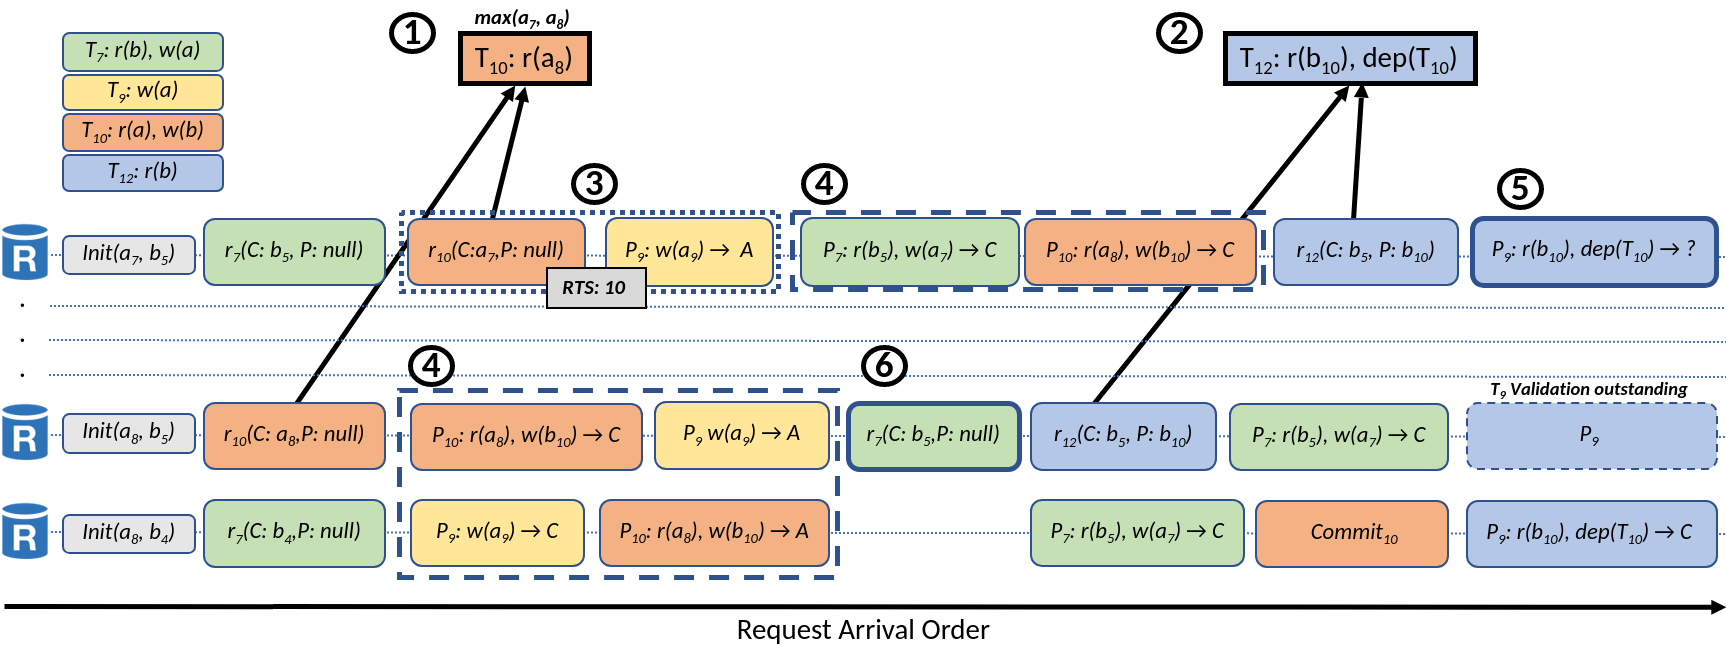
\includegraphics[width= \textwidth]{./figures/MVTSOLargeFont.png}
\end{center}
\caption{\emph{MVTSO behavior for different replica processing orders}. $r_x(C : a_y ,P : a_z)$ denotes that transaction $T_x$ (x being the timestamp of a transaction in this example) reads the version $y$ of object a written by committed transaction $T_y$ and version $z$ from tentative prepared transaction $T_z$. $P_x(RS,WS,DEP)$ denotes a transaction $T_x$'s prepare request (i.e. the validation check) for respective ReadSet (RS), WriteSet (WS) and Dependenc Set (DEP), and $\rightarrow C / A$ denotes the local replica validation outcome (Commit/Abort).} 
\label{fig:MVTSOEX}
\end{figure*}

\par \textbf{MVTSO.} Our starting point is Multiversioned Timestamp Ordering (MVTSO), a concurrency control scheme which prescribes a serialization order by assigning a speculative timestamp \textit{before} execution \cite{bernstein1983multiversion, reed1983implementing, su2017tebaldi}. In MVTSO, read operations return the latest written version smaller than the readers' timestamps. Respectively, writers attempt to create new versions at their timestamp, but must abort if a higher timestamped read would have "missed the write" by reading a prior version. A transaction may commit only, if all read-write dependencies have committed.

\iffalse
\fs{cut the whole following paragraph?} \la{Yes, I would cut it} This allows us to a) only classify concurent read/write operations as conflicting if their execution results violate the timestamp order (Fig. \ref{fig:MVTSOEX}: 4 bottom), and b) avoid write/write conflicts alltogether. 
When speculative execution results match the pre-defined timestamp order, no aborts are necessary (Fig. \ref{fig:MVTSOEX}: 4 top). \sys{}'s challenge is therefore to a) assign appropriate timestamps and b) coordinate execution in a way that maximizes such coherence; the presence of Byzantine participants (clients/replicas) complicates this.

In MVTSO, reads operations return the latest written version smaller than the readers' timestamps, while writers attempt to create new versions at their timestamp, but must abort if a higher timestamped read would have "missed the write" by reading a prior version. A transaction may commit only, if all read-write dependencies have committed.
\fi

When \sys{}'s speculative execution results match the pre-defined timestamp order, no aborts are necessary (Fig. \ref{fig:MVTSOEX}: 4). \sys{}'s challenge is therefore to a) assign appropriate timestamps and b) coordinate execution in a way that maximizes such coherence; the presence of Byzantine participants (clients/replicas) complicates this.

\par \textbf{Byzantine resilience.} Read operations in \sys have the following sub-goals: \one Correct clients should read valid data, i.e. experience read integrity, \two Correct clients should read fresh data, i.e. minimize staleness and hence maximize commit chance, and \three Reads must provide the context necessary to potentially complete observed write state. 
Clients validate the integrity of reads by requiring replicas to provide a proof of validity, which consists of a set of signatures confirming committment, or if not yet existant, a set of  $f+1$ replica's tentative commit endorsements \fs{maybe cut this second part, since it will become redundant}. Moreover, to guarantee that clients do not read maliciously stale data from their local replica, \sys encourages clients to read the latest version across $\geq f+1$ replicas (Fig. \ref{fig:MVTSOEX}: 1,2).
Avoiding Byzantine influence comes at a cost: Read operations require a synchronous, potentially WAN \fs{or just remote - i.e. not local}, rountrip. 

MVTSO intuitively synergizes well with \sys{}'s potenially WAN remote reads as reading from a fixed timestamp helps speculative readers observe consistent snapshots, even when execution is long and consequently interleavings are frequent (Fig. \ref{fig:MVTSOEX}: 6). \fs{at the price of experiencing serializability instead of strict serializability - that is only the case if your timestamps are outdated}.

While we assume that clocks are loosely synchronized across correct participants, Byzantine participants may diverge arbitrarily and propose excessively high timestamps. A simple solution is to bound time-stamps by querying the median time from a Quorum of replicas and including replies as proof \cite{bazzi2004non, bazzi2018clairvoyant}. To side-step the additional overheadd that a dedicated timestamping phase incurs, we compromise by allowing clients to optimistically select their own timestamps, but reject request timestamps above a threshold at all correct replicas, thus incentivising clients to select bounded, close to real-time, timestamps. 

In traditional MVTSO, writes become visible to successive, higher timestamped, reads immediately. However, in the presence of Byzantine clients this is undesirable, as it allows clients to issue write operations without the intention of ever committing a transaction. Thus, any correct clients' read that observes, and consequently depends on a Byzantine clients write may be blocked indefinitely.
%Allowing other clients to preemtively commit outstanding write operations is infeasible, as the remaining transaction procedure is known only to the issuing client, while conceiding pessimistic abort permission empowers Byzantine participants to obstruct any correct clients' writes. 
\sys reconciles this dilemma by deferring all database updates until execution is complete and the client prepares the transaction for commitment. 
% Concretely, \sys clients buffer all write operations, and submit them only when attempting to commit the transaction, thereby enabling other \sys client to orderly complete Validation and Writeback steps.\\
\la{This needs to be better explained} \fs{took a pass:}
Clients in \sys distinguish explicitly between writes \textit{committed} across all involved shards and tentative writes \textit{prepared} at a single shard: While clients accept all verifiable \textit{committed} version from a single replica, they accept \textit{prepared} versions only when endorsed by $f+1$ replicas. This ensures that a) at least one correct replica believes that the write can commit, and hence is worth observing, and b) that Byzantine replicas and clients cannot collude to violate Byzantine independence by reactively inventing versions. \fs{such invented transactions could be designed to be guaranteed to abort: I.e. by claiming to have read an out-dated version. The write versions could be engineered to be perfectly at the bound of the read timestamp, such that it is guaranteed to be chosen}\\
Finally, \sys replicas evaluate writes for conflicts by maintaining a Read Timestamps (RTS) for each locally processed read (Fig. \ref{fig:MVTSOEX}: 3). While this allows un-prepared reads to elicit external effects, these affect only concurrent transactions with smaller timestamps and can be bypassed by re-trying a transaction. To nonetheless limit recurrent abuse, we discuss a personalized lease mechanism to limit Byzantine influence in section Y.z (Optional Modifc). \fs{or just do it here in 1-2 sentences. We do not implement this though.}



\subsection{Execution interface}
Client applications execute transactions via the following interface. A TX object \textit{TXObj $\coloneqq$ (SeqNo, ClientID, InvolvedShards, ReadSet, WriteSet, Dependencies)}, records the state necessary for Validation.

\iffalse
\begin{figure}
\begin{center}
\includegraphics[width= 0.5\textwidth]{./figures/TxState.png}
\end{center}
\caption{Transaction execution state}
\label{fig:Txstate}
\end{figure}
\fi

\textbf{Begin()} A client begins a transaction by optimistically choosing a timestamp \textit{TS $\coloneqq$ (Time, ClientID)} that defines a total serialization order across all clients.  \\
\textbf{Write(key, value)}. A client buffers the write: \textit{WriteSet = WriteSet $\cup$ (key, value)}\\
%%%%%%%%%Read protocol%%%%%%%%%%%
\textbf{Read(key, TS, RQS)} 
If \textit{key $\in$ WriteSet} a client returns the buffered write value. Otherwise, the client conducts a remote read for given hyperparameter Read Quorum Size (RQS):

\fbox{\begin{minipage}{23em}

\textbf{1: C} $\rightarrow$ \textbf{R}: Client sends read request to Replicas
\end{minipage}}\\
%Improve RQS formulation
A client broadcasts a read request  $m = (Read, key, TS)_c$.
\iffalse
 to $RQS$ different replicas. Note, that in order to guarantee $\geq RQS$ replies a client might need to send up to $f$ additional requests to compensate for unresponsive/faulty participants ($max(|Replies|) \leq n-f$). 
\fi
\fs{Optimization: A client sends only to RQS+f to receive RQS many replies}

\fbox{\begin{minipage}{23em}
\textbf{2: R} $\rightarrow$ \textbf{C}: Replica processes client read and replies
\end{minipage}}\\
A replica authenticates the client\footnote{Byzantine replica may ignore read access control. Solving this problem is beyond the scope of this work; we defer to existing solutions \cite{basu2019efficient}.}, and enforces a local timestamp threshold. \fs{this can probably be shortened:} It returns a signed message \text{$\langle \textit{ReadReply, Committed, Prepared} \rangle _R$}, where $Committed \coloneqq (value, version, proof)$ represents the value-version pair with largest committed write version smaller than TS and a proof of commitment,  and $Prepared \coloneqq (value, version, TxID', deps)$ the respective largest uncommitted value-version pair, the associated transaction ID, and the latter transactions potentially uncommitted read-write dependencies. Moreover, a Replica stores a new read timestamp (RTS) for the key: $RTS(key) = RTS(key) \cup TS$ (Fig. \ref{fig:MVTSOEX}: 3). 
\fs{a replica may include a set of prepared values to increase likelihood of client receiving f+1 matching}

\fbox{\begin{minipage}{23em}
\textbf{3: C} ($\rightarrow$ \textbf{R}): Client receives read replies 
\end{minipage}}\\
A client waits for $\geq RQS$ read replies and chooses the biggest valid result \textit{(value, version) $= max_{valid}$(\{Committed\},\{Prepared\}} (Figure \ref{fig:MVTSOEX}: 1,2). A \textit{Committed} tuple is valid, if the proof confirms commitment, wheras a \textit{Prepared} is valid iff there exist $f+1$ matching \textit{Prepared$_r$}. The client adds the version to its read set \textit{ReadSet = ReadSet $\cup$ (key, version)} and additionally claims a dependency if it was a \textit{Prepared} version: \textit{Dep = Dep $\cup$ \{f+1 $\times$ Prepared$_r$ \}} . 

\fs{la: finds the use of commit in both exec and validation confusing. Is it unclear that this refers to application here?}
\textbf{Commit()} A Client terminates its execution, and computes a unique transaction identifier based on final execution object and its timestamp: $TxID \coloneqq (H(TxObj, TS)$, thus preculding Byzantine participants from equivocating transaction contents. It then initiates the Validation Phase by issuing a 2PC-Prepare requests to each involved shard.
%What if a byz doesnt send to all involved shards? It will be visible on some shard and hence an correct client can obtain the full TX. See Hierarchical IDS in Protocol.tex

\textbf{Abort()} A client terminates execution, and broadcasts a request to release all acquired Read Timestamps (RTS). Since writes in \sys are deferred, no other rollback action is necessary.


We briefly discuss some implications of the choice of Read Quorum Size (RQS). Following cases may be distinguished: \one \textbf{$RQS = 1$} A client may read committed data from just \textit{trusted} replica (at the risk of reading stale data) to reduce execution latency and consequently minimize conflicting interleavings. \two \textbf{$RQS \geq f+1$} \sys{}'s recommended minimal mode of operation. While side-stepping maliciously stale reads, it is still possible to read (arbitrarily) stale data due to replica inconsistency, caused by either asynchrony or partial transaction replication by a Byzantine client.
\three \textbf{$RQS \geq \frac{n+f+1}{2}$} When reading from a Quorum of sufficient size to overlap with any Validation Quorum (ref section Validation) in at least one correct replica, a client guarantees, that no more \textbf{additional} (beyond previously observed) conflicting writes can be admitted, since such a Quorum of acquired RTS acts as a read-lock. 

\iffalse
Trusting only $f+1$ matching prepared writes has the beneficiary side effect of allowing us to include only transaction identifiers as dependencies, rather than the full transaction, since it is guaranteed that at least one correct replica has stored the transaction. Thus, in the failure free scenario, where clients need not complete transactions $in Dep$, \sys minimizes the meta-data overhead that the recovery protocol imposes.
\fi

We remark that, consistent with Byz-Isolation, \sys allows Byzantine clients to fabricate and (permissibly) submit arbitrary reads; Byzantine clients may \textit{choose} whether to read legal, or even real data.  \sys does, however, enforce that Byzantine clients cannot (undetectably) fabricate dependencies by requiring a proof of $f+1$ matching prepared writes. This precludes Byzantine clients from indetectibly stalling their own transactions and consequently obstructing liveness for consecutive descendant (second degree...) dependencies.
Furthermore, this allows \sys to include only transaction identifiers as dependencies, rather than the full transaction, thereby minimizing the common path overhead. The full transaction can be acquired from an correct replica when necessary. We discuss how to complete stalled or slow transactions in section Y (Granting Liveness).





%
\subsection{Validation Check}

Algorithm \ref{mvtso} shows the necessary validation check to preserve Byzantine-Serializability. 
Given a transactions prepare request the validation check returns an Abort vote if a conflict has been detected, and Commit otherwise. 
When execution results match the timestamp order, there are no conflicts (Fig. \ref{fig:MVTSOEX}: 4 top). For each read, a replica verifies that it has not voted to commit a conflicting write (Algorithm \ref{mvtso}, line 3-7). Conversely, for each write, a replica confirms that there exist no previously accepted reads (line 8-10), and no ongoing read transactions (line 11-12) that conflict. Fig. \ref{fig:MVTSOEX}: 4 shows both non-conflicting and conflicting interleavings.
If there are no conflicts, a replica tentatively \textit{prepares} a transaction, making its writes visible and evaluating future transactions against it for conflicts. Regardless of the outcome, a replica garbage collects all Read Timestmaps (RTS) associated with the transactions reads.
It then waits for necessary dependencies (uncommited writes that were read) to be resolved (Figure \ref{fig:MVTSOEX}: 5). We remark, that the concurrency control check is serialized and executed atomically for each transaction.

\begin{theorem}
The set of transactions for which the MVTSO-Check returns Commit is Byzantine-Serializable. 
\end{theorem}
\begin{proof}
See TR.
\end{proof}

\begin{algorithm}
\caption{MVTSO-Check(TX, TS)}\label{mvtso}
\begin{algorithmic}[1]
\If{\textit{$TS > localClock + \delta$}} %  || $TS < lowWM$ || $\exists d \in dep: d.TS < lowWM$} } dont mention garbage collection part here, it only confuses
\State \Return Abort
\EndIf

\For{\textit{$\forall key,version \in \textit{TX.RS}$}}
        \If{$ \exists TX2 \in Committed \cup Prepared: key \in \textit{TX2.WS} $ \newline
        \hspace*{2em} $\land \, version < \textit{TX2.TS} < TS$}  
          \State  \Return Abort, \textit{TX2, (TX2.CommitProof)}  
         \EndIf  
\EndFor

\For{\textit{$\forall key \in \textit{TX.WS}$}}
        \If{$\exists TX2 \in Committed \cup Prepared:$ \newline 
        \hspace*{2em} $\textit{TX2.RS[key].version} < TS < TX2.TS$} 
          \State  \Return Abort, \textit{TX2, (TX2.CommitProof)}
         
        \EndIf
        \If{$\exists RTS \in key.RTS: RTS > TS$} 
          \State  \Return Abort
       \EndIf
\EndFor
\State Prepared.add(TX) 

\While{$\exists d \in dep: d \notin CommitLog \cup AbortLog $)}
\State Suspend
\EndWhile

%structure it in a way that is better
\For{\textit{$\forall d \in dep$}}
		\If{$ d \in AbortLog $}
		\State	Prepare.remove(TX)
		\State \Return Abort, \textit{(TX2.AbortProof)}
		\EndIf
\EndFor
\State \Return Commit
\end{algorithmic}

\end{algorithm}

In order to perform the MVTSO-check, a replica maintains several data strucutres: \one It stores read timestamps, read versions alongside the multiversioned write stores for committed and tenative transactions respectively, to provide efficient evaluation of conflicts.
\two In order to confirm dependency outcomes, replicas log proofs for completed transactions in respective Commit and Abort Log sets, that together induce the ledger of all processed transactions. 
\three To avoid busy waiting when dependencies are not yet resolved, a replica temporarily suspends the MVTSO-check for the current transaction, allowing it to process other transactions pending validation. To facilitate this, it keeps track of an additonal transaction to dependents mapping that allows to identify and resume all suspended MVTSO-checks associated with dependents of a completing transaction.

\iffalse

\textit{Aside:} Consistent with our definition of Byzantine-Isolation, byzantine clients may issue ficticious Read-Sets comprised of arbitrary read versions and values. However, these have only limited external effect on concurrent writes. We distinguish two extreme cases: 1) $read.version \rightarrow 0$: This case is equivalent to simply reading stale data, and effectively reduces MVTSO to TSO as conlflicts are evaluated only on basis of the transaction timestamps (i.e. Abort write if: write.TS < read.TS). 2) $read.version \rightarrow read.TS$: In this case there are no conflicts as a write is never "missed" by a previous read.
\fi

In the following section we will show how to design a replicated validation scheme that upholds Isolation guarantees and reaches a single shard decision, even when replicas within a shard validate in different orders.


%%-------------------------------------------------------------------------------
\subsection{Validation Phase}
%-------------------------------------------------------------------------------

In order to facilitate atomic committment across all shards involved in a transaction \sys clients invoke a Prepare request, inquiring each shard to validate the transaction for conflicts and cast a 2PC vote. Shards in \sys are replicated for fault tolerance.

\fs{idk where to put this and whether to mention at all - but we do want to state that there exists a version with 3f+1 (minimal replication degree) that implements the same ethos }
\sys comes in two different flavors, \sys{}3 and \sys{}5 respectively, that rely on varying replication degrees, but implement the same design. \sys{}3 requires $n=3f+1$ replicas \fs{, the minimum bound necessary for BFT SMR?,} per shard to guarantee consistency in the presence of $\leq f$ byzantine replicas. \sys{}5 reduces both latencies during failure free execution and complexity during recovery. \footnote{We believe that consortiums with high performance requirements or high replication degrees are respectively comfortable with paying for additional replicas or tolerating a lower fraction (1/3 vs 1/5) of failures}
For the simplicity of exposition we discuss \sys{}5 for the remainder of the paper, and defer to section X \fs{and/or TR} to describe differences in \sys{}3. In the following, we outline \sys 's execution (unaffected by replication degree), validation and writeback protocols.

The goals of the Validation phase are threefold: \one It must decide on a single, durable vote per-shard that maintains Byzantine Serializability (henceforth we refer to this as a \textit{shard-decision}), \two It should be leaderless, and not enforce unecessary ordering for commutative, non-conflicting transactions, and \three It must preserve independent operability. \fs{needs to refer to the fallback}

Satisfying these goals requires ovecoming several challenges. In order to maximize parallelism and embrace partial ordering, \sys allows replicas to process requests out of order. Consequently, replicas may temporarily diverge, and hence return different validation results. Such divergence must be reconciled in a way that maintains Isolation, but not overly conservatively in order to bound the impact of byzantine participants and maximize likehlihood to commit. \sys designates clients as validation coordinator for its own transactions, thus omitting a dedicated replica leader. %The respective protocol must tolerate client failures such as crashes, omission/stalling, equivocation, or replays and allow for consistent recovery. 

The Validation protocol can be broken down into two functionalities: Voting and Logging.
Since \sys replicas may process requests in different order, they must reach consensus on a joint  decision. To do so, they cast a vote for their local validation result, which are subsequently democratically aggregated into a decision. In the case of Indicus, the client acts as the transaction coordinator who aggregates and relays results (along with necessary evidence).
In order to maintain consistency in the presence of failures (no two honest replicas finalize different Commit/Abort decisions), this decision must be durable and unique, guaranteeing that a replay of any Writeback is idempotent. However, since a byzantine coordinator cannot be trusted to durably store a decision, nor could we retain liveness during a crash or partition, \sys demands clients to \textit{log} the decision at replicas before returning.
 

The voting step requires a single round-trip to all replicas, whereas the logging phase requires at most one round-trip \fs{in Indicus5 and at most two round-trips in Indicus3.}. When execution is fault- and contention free transactions can be committed on the \textit{Fast-Path} in a single-round trip as an explicit logging round is not necessary.


%%%%%%%%%% protocol
To describe how the protocol operates in detail we follow a single-shard transaction through the system:

\fbox{\begin{minipage}{23em}
\textbf{(1: C $\rightarrow$ R)}: Client sends Prepare request to all Replicas within the Shard.
\end{minipage}}\\
Upon deciding to Commit in the Execution phase, a Client initiates Validation by sending a message $Phase1 \coloneqq \langle Prepare, TxID, TX \rangle_{\sigma_c}$ to all Replicas.

\fbox{\begin{minipage}{23em}
\textbf{(2: R $\rightarrow$ C)}: Replica receives validation request, processes it and returns vote to Client.
\end{minipage}}\\
A replica validates Timestamp and Dependency integrity of the request. It then evaluates Read and Write Sets for Isolation conflicts against its local state using the MVTSO Concurrency Control Check (CCC), as shown in algorithm 1. It returns a message $Phase1R \coloneqq \langle TxID, vote \rangle_r$, and optionally evidence in case it voted to Abort.

\underline{Additional subtlelties}: 
A replica never changes its Voting decision, because re-execution could leave to different results. Once the MVTSO-Ceck completes (i.e. there are no blocking dependencies), a replica starts a timer to monitor the clients progress.

\fbox{\begin{minipage}{23em}
\textbf{(3: C)}: Client waits for vote replies.
\end{minipage}}\\
A client waits for at least $n-f$ ($4f+1$ in Indicus5) distinct replica votes, or more, up to a system specified timeout. 

\fbox{\begin{minipage}{23em}
\textbf{(3a: C)}: Client receives Threshold of matching votes and returns to application. Proceeds to Writeback
\end{minipage}}\\
In any of the following 3 cases, a client may short-circuit waiting for additional votes and omit a dedicated Logging round:
\begin{enumerate}
\item \textbf{$1$ Abort vote w/ Conflicting TX \& CommitCertificate}: A conflict with a commited transaction. The client validates the integrity of the CommitCertificate and returns the shard decision $(TxID, Abort, \langle ConflTX \rangle_{CC})$. 
\item \textbf{$3f+1$ Abort votes w/ Conflicting TX}: A conflict with a prepared, but not yet committed transaction. The client returns the shard decision $(TxID, Abort, \{\langle AbstainVote\rangle_r\})$. 
\item \textbf{$5f+1$ Commit votes}: No conflicts. The client returns the shard decision $(TxID, Commit, \{\langle CommitVote \rangle_r\}$
\end{enumerate}
Any of such Quorums forms a \textit{Shard-Certificate} and proves the decision. A client uses this Certificate to return to its application and issue the Writeback.

\fbox{\begin{minipage}{23em}
\textbf{(3b: C $\rightarrow$ R)}: Client receives divergent results and suggests a consistent decision to Replicas for Logging
\end{minipage}}\\
If a client does not receive the necessary thresholds of votes to return, it must continue on the \textit{Slow-Path}. To do so, it aggregates the votes according to following decison rule:
If there exists a $CommitQuorum \coloneqq \frac{n+f+1}{2}$ of Commit Votes, the Slow-Path decision is Commit, otherwise it is Abort.
A client broadcasts a message $Phase2 \coloneqq (TxID, decision)_c, \{\langle votes \rangle_r\}$.

\underline{Additional subtlelties}: A client forwards a Quorum of $\geq n-f$ votes to the replicas in order to prove the Slow-Path decision is consistent with Isolation guarantees. Note, that a byzantine client may equivocate the decision by relaying different Quorums.

\fbox{\begin{minipage}{23em}
\textbf{(4: R $\rightarrow$ C)}: Replicas receive, validate and echo decision
\end{minipage}}\\
A replica confirms that the Decision matches the Quorum by evaluating the decision rule itself and adopting the decision. It then returns the decision to the client by sending $Phase2R \coloneqq \langle TxID, decision \rangle_r$. Importantly, a replica never changes its decision.

\fbox{\begin{minipage}{23em}
\textbf{(5: C)}: Client returns shard-decision to application and proceeds to Writeback
\end{minipage}}\\
A client waits for a Quorum of $n-f$ matching $Phase2R$ messages. Such a Quorum forms a \textit{Shard-Certificate} and proves the decision. A client uses this Certificate to return to its application and issue the Writeback.

\underline{Additional subtlelties}: If a client equivocated, it will never receive a Shard-Certificate. An honest client however, is guaranteed to receive matching Phase2 replies. 

We consider a decision (Commit, Abort) to be \textit{logged} when it is possible for some Shard-Certificate to exist, i.e. as soon as the necessary certificate Quorums exists at some Replicas.
Figure \ref{fig:FigureSP} summarizes the relevant nomenclature.

\begin{figure}
\begin{center}
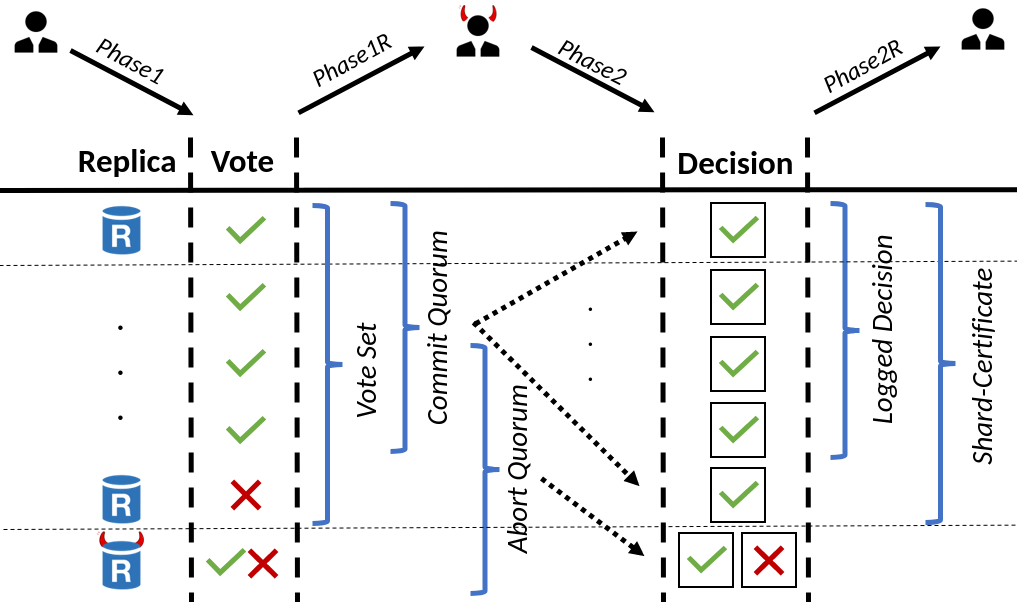
\includegraphics[width= 0.5\textwidth]{./figures/Nom2.png}
\end{center}
\caption{Validation Nomenclature, Slow-Path. Note, that a byzantine client may equivocate Phase2 decisions by including Commit and Abort Quorums respectively. Byantine replicas may store multiple votes and decisions.}
\label{fig:FigureSP}
\end{figure}

\subsubsection{Correctness}
We show, that a \textit{logged} decision is final:
\begin{theorem}[Saf]
A logged decision is durable, and there can ever exist \textbf{at most one} logged decision.
\end{theorem}
\begin{proof}
See TR.
\end{proof} 

Note, that since replicas never change their decision, it is possible for there to never be any logged decision if a byzantine client equivocated its Slow-Path Quorums. In order to reconcile this, we design and discuss a recovery mechanism in section X which relaxes the requirement on persisting a decision.  


\begin{theorem} 
Indicus maintains \textit{Byzantine-Serializability}.
\end{theorem}
To prove that this is the case, we show that for any two conflicting transactions, at most one can be committed.
\begin{proof}
See TR.
\end{proof}

\begin{theorem} 
Indicus maintains Byzantine Independence in the absence of network adversary.
\end{theorem}

We show, that once a Client submits a transaction for validation, the result cannot be unilaterally decided by any byzantine participant, be it client or replica.
\begin{proof}
See TR.
\end{proof}

%%-------------------------------------------------------------------------------
\subsection{Writeback}
%-------------------------------------------------------------------------------



%\subsection{Multi-sharding}

and Multi-shard 2pc

- Optimization: Single shard logging


%%-------------------------------------------------------------------------------
\subsection{Failures}
%-------------------------------------------------------------------------------
- Fallback: election (only starts if not waiting on another dep to avoid early eviction), views, resolution, subtelties with mvtso (block because of dep), necessity even without dependencies. Interested clients, write-back multishard. garbage collection
- Fallback requires an extra round in order to learn about current views to start viewchange, but thats ok: Its co-function with learning about full TX, and checking for existing certificates. Timeout invocation is concurrent with p1 message.



%%-------------------------------------------------------------------------------
\section{Further optimizations}
%-------------------------------------------------------------------------------


\fs{the current writeback might be unecessary to explain, since we implement the below anyways... Perhaps merge writeback and this subsection}
\par \textbf{Shard Logging} When transaction execution touches multiple shards validation can incur redundant explicit logging overhead. When a Slow-Path is necessary to arrive at a logged decision on S different shards, bandwith is wasted. Consider an example in which $S-1$ shards attempt to log the decision Commit, while a single shard attempts to log an Abort decision. If the latter shard succeeds, the effort of the remaining shards was in vain. \fs{Moreover, logging is always bottlenecked by the slowest shard. }
The culprit of this phenomenon is the delayal of Two-Phase-Commit (2PC) until the Writeback phase. By preemptively making a 2PC decision \textbf{before} logging we can avoid this redundancy. We remark, that even when when all shards agree on a decision, this saves redundant coordination. \fs{This does not work for Atomic Broadcast! In AB, the voting only happens AFTER the tx has already been logged (i.e. the order has been durably replicated)}

Concretely, we designate \textbf{one} involved shard as \textit{logging Shard} $=$ \textit{involvedShards[TxID \% |involvedShard|]}, while all other shards remain responsible only for Voting. \changebars{}{The logging Shard can be determin via a determinsitic function over the \textit{involved Shards}. A simple load balanced solution may select $loggingS = involvedShards[TxID \% |involvedShard|]$}. \changebars{}{Figure \ref{fig:SingleShardOpt} shows a comparison and the revised structure. dont use this figure in actual paper} In order to log a decision, Phase1R Quorums \fs{aka shard votes} from all involved shards are required. We modify step 3 of the Validation protocol accordingly:

\fbox{\begin{minipage}{21em}
\textbf{Validation (3: C)}: Client waits for vote replies from all involved Shards.
\end{minipage}}
A client aggregates a per-shard decision for each shard according to the \textit{CommitQuorum} rule. If all shard-decisions are Commit, it attempts to log a Commit decision by sending $Phase2 \coloneqq (TxID, Commit, S \times \{CommitQuorum\}$ to all replicas in the designated logging Shard. If a single shard-decision is Abort, it stops waiting for other shard-decisions and attempts to log an Abort decision by instead sending $Phase2 \coloneqq (TxID, Abort, AbortQuorum)$. 

\underline{Additional subtlelties:} A client can go Fast-Path and return to the Writeback phase immediately only if Fast-Path Quorums were received for all shards. 

The remaining Validation protocol proceeds identically to the multi-shard version. Notice, that when only a single shard is involved, no adjustments were made. The Writeback phase instead, may proceed with just the single certificate from the logging Shard


The Fallback protocol is adjusted accordingly: A fallback replica need (and can) only be elected on the logging Shard, simplifying reconciliation and reducing the cost for interested clients. 
To further reduce unecessary load, a client may attempt to first inquire whether decisions exists at the logging shard (Fallback protocol step 1 \& 2), before sending $Rec-Phase1$ messages to all shards in order to gather votes itself (Fallback protocol step 1). 

\iffalse
\begin{figure*}
\begin{center}
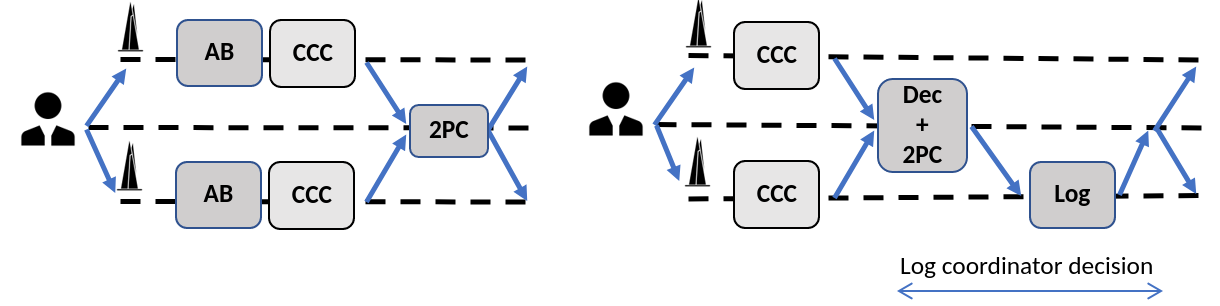
\includegraphics[width= \textwidth]{./figures/SingleShard.png}
\end{center}
\caption{Single Shard Optimization}
\label{fig:SingleShardOpt}
\end{figure*}
\fi

\par \textbf{Batching}
To amortize cryptographic overheads we introduce message batching. However, unlike leader based systems, in \sys there exists no central sequencer that may batch request. Instead, \sys implements message batching at the replicas by batching $b$ messages, generating a merkle tree \cite{merkle1987digital}, and signing only the root hash, thus reducing signing overheads from $O(b)$ to $O(1)$ per batch. The merkle hash tree allows replicas to respond to individual clients by including only the single client-addressed message and $log(b)$ additional hashes. We note, that since replicas receive requests out of order, their batches are not consistent. Consequently, a client must aggregate hashes and signatures from different merkle trees to forward as proofs (Phase2 and Writeback messages include $O(n)$ signatures and hashes) .
In order to reduce verification overheads from $O(n*b)$ to $O(n)$, replicas cache previously verified signatures by storing a mapping from signature to merkle hash roots. For following message verifications, a replica can omit de-computing the signature, and must only re-compute and compare the merkle root based on the hashes included in the proof.

\iffalse
- amortize signature cost
- unlike leader based, there is not an obvious sequencer to batch
- instead we batch signature generation at replica. Because they can be out of order these batches are different. Also do not want to send the whole batch (b* hashes) to every client. Instead we use a merkle tree and send only the root sig + log(b) hashes. (this means that we had to do 2*b hashes during signature gen, but we only do b*log(b) hashes at generation instead of b*b. OR: could send whole batch of  messages --> huge message + hashing cost..
- Cache already validated signatures at replicas and only recompute the hash to see whether it matches. This reduces verification by a factor of b (effectively only verifying for the first message from the batch).
\fi

\par Other non impelmented opts: in TR.

 
